\documentclass[tikz]{standalone}
\begin{document}
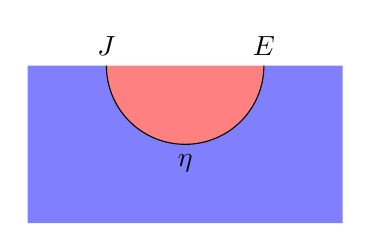
\begin{tikzpicture}
\coordinate (eta) at (2.000, 1.000);
\coordinate (J) at (1.000, 2.000);
\coordinate (E) at (3.000, 2.000);
\fill[blue!50](0.000, 0.000) -- (0.000, 2.000) -- (J) to[out=-90, in=180] (eta) to[out=0, in=-90] (E) -- (4.000, 2.000) -- (4.000, 0.000) -- cycle;
\fill[red!50](E) to[out=-90, in=0] (eta) to[out=180, in=-90] (J) -- cycle;
\path[draw=black!100](E) to[out=-90, in=0] (eta) to[out=180, in=-90] (J);
\node[below] at (eta) {$\eta$};
\node[above] at (J) {$J$};
\node[above] at (E) {$E$};
\end{tikzpicture}

\end{document}
